\documentclass[conference]{IEEEtran}

% *** GRAPHICS RELATED PACKAGES ***
\usepackage{graphicx}
\usepackage{pgfplots}
\usepackage{float}
\usepackage{caption}
\usepackage{subcaption}

% *** MATH PACKAGES ***
\usepackage{amsmath}
\usepackage{amssymb}
\usepackage{bm}
\usepackage{amsthm}

% *** SPECIALIZED LIST PACKAGES ***
\usepackage{algorithm}
\usepackage{algpseudocode}

% *** ALIGNMENT PACKAGES ***
\usepackage{array}

% *** PDF, URL AND HYPERLINK PACKAGES ***
\usepackage{url}

% *** TABLES PACKAGES ***
\usepackage{booktabs}
\newcommand{\ra}[1]{\renewcommand{\arraystretch}{#1}}

% *** USER DEFINITION ***
\newtheorem{Remark}{\bf Remark}

\begin{document}

\title{Data Driven Hyperparameters Optimization of One-Class Support Vector Machines for Anomaly Detection in Wireless Sensor Networks}

\author{\IEEEauthorblockN{Van Vuong~Trinh and Kim Phuc~Tran}
\IEEEauthorblockA{Division of Artificial Intelligence,\\Faculty of Information Technology,\\ Dong A University, Danang, Vietnam\\Email: vanvuong.trinh@gmail.com, phuctk@donga.edu.vn}
\and
\IEEEauthorblockN{Truong Thu Huong}
\IEEEauthorblockA{Department of Telecommunication Systems,\\School of Electronics and Telecommunications,\\Hanoi University of Science and Technology, Hanoi, Vietnam\\Email: huong.truongthu@hust.edu.vn}}

\maketitle

\begin{abstract}
One-class support vector machines (OCSVM) have been recently applied to detect anomalies in wireless sensor networks (WSNs). Typically, OCSVM is kernelized by radial bais functions (RBF, or Gausian kernel) whereas selecting hyperparameters is based upon availability of anomalies, which is rarely applicable in practice. This article investigates the application of OCSVM to detect anomalies in WSNs with data-driven hyperparameters optimization. Specifically, the information of the farthest and the nearest neighbors of each sample is used to construct the objective cost instead of labeling based metrics such as geometric mean accuracy (G-mean) or area under the receiver operating characteristic (AUROC). The efficiency of this method is illustrated over the IBRL dataset whereas the resulting estimated boundary as well as anomaly detection performance are comparable with existing methods. 
\end{abstract}

\begin{IEEEkeywords}
one-class support vector machines,  anomaly detection, wireless sensor networks, Gaussian kernel, parameters selection.
\end{IEEEkeywords}

\IEEEpeerreviewmaketitle

\section{Introduction}

WSNs are composed of a large number of sensor nodes that can communicate the information gathered from a monitored field through wireless links to monitor physical or environmental conditions, such as temperature, vibration, pressure, motion, etc. and to cooperatively pass their data throughout the network. WSNs are an emerging and very interesting technology applied to different applications including industrial processes, monitoring and control, machine health monitoring, healthcare applications and traffic control. WSNs will be an integral part of our lives, more so than the present-day personal computers (see \cite{Xie2011}). Due to the deployment of a large number of sensor nodes in uncontrolled or hostile environments, data measured and collected by WSNs is often  unreliable. This will affect the modeling and scientific reasonable inference. Thus, it is significant that the anomaly of sensor node is detected in order to obtain accurate information, therefore make effective decisions by information gatherered (see, for instance, \cite{sharma2010sensor}).\\

Anomaly detection is a method to identify whether or not a metric is behaving differently than it has in the past, taking into account trends. This is implemented as one-class classification since only one class is represented in the training data. Several methods have been proposed to solve the one-class classification problem which can be classified into three main types the density estimation, the boundary methods and the reconstruction methods. In literature, a variety of anomaly detection techniques have been developed for certain application domains such as security systems, fraud detection and statistical process monitoring, for example, see \cite{ilonen2006gaussian}, \cite{clifton2011novelty}, \cite{Tran2015a}, \cite{Tran2015b}, \cite{Chandola2016}, \cite{Tran2016} and \cite{Tran2016c}. Recently, there have been growing interests in applying machine learning approaches for anomaly detection in WSNs. For further details see, for instance, \cite{sharma2010sensor}, \cite{Xie2011}, \cite{Rajasegarar2014}, \cite{Chandola2016}, and\cite{feng2017new}. Recently, \cite{shahid2015one} presented a detailed analysis of various formulations of OCSVM, like, hyper-plane, hyper-sphere, quarter-sphere and hyper-ellipsoidal to separate the normal data from anomalous data for wireless sensor networks in harsh environments.\\

In this contribution, we study a data driven algorithm based on OCSVM  for anomaly detection in WSNs. We test the performance of the algorithm on real data set obtained from a WSN deployment at the Intel Berkeley Research Laboratory. The remainder of the paper is organized as follows: in section \ref{sec:OCSVM}, some necessary background on OCSVM are introduced; in section \ref{sec:implementation}, the anomaly detection approach in WSNs is defined; section \ref{sec:Illustrative} presents an illustrative example, and finally, some concluding remarks and recommendations are made in section \ref{sec:concluding}.

\section{One-Class Support Vector Machines and Gaussian Kernel}\label{sec:OCSVM}

In this section, we briefly review one-class support vector machines (OCSVM) \cite{scholkopf2001estimating} and the Gaussian kernel.

OCSVM is used to estimate the support of a distribution.
Notationally, let us consider a data set $\{\mathbf{x}_1,\mathbf{x}_2,\ldots,\mathbf{x}_i, \ldots,\mathbf{x}_N\}$, 
with each $\mathbf{x}_i\in \mathcal{R}^D$ belonging to a given class of interest (named target class). 
The basic idea behind the OCSVM is to separate data from the origin by finding a hyperplane with maximum margin separation from
the origin. In order to deal with nonlinearly problems, the hyperplane is defined in a high-dimensional Hilbert feature space $\mathcal{F}$ where
the samples are mapped through a nonlinear transformation $\Phi(.)$. We will work only a kernel function $k(\mathbf{x},\mathbf{y})$ instead of the scalar 
product $(\boldsymbol{\Phi}(\mathbf{x}).\boldsymbol{\Phi}(\mathbf{y}))$. To separate the data set from the 
origin, \cite{scholkopf2001estimating} solved the following quadratic program:
\begin{subequations}\label{euq:ocsvm}
\begin{align}
\underset{
	\begin{array}{c}
		 \mathbf{w}, \mathbf{a}, \boldsymbol{\xi}, \rho
	\end{array}}{\text{Minimize }} & \frac{1}{2}\left|\left| \mathbf{w}\right|\right|^2 + \frac{1}{\nu N}\sum_{i=1}^N\xi_i -\rho\\
	\label{euq:constraints}
\text{Subject to } &  (\mathbf{w}.\Phi(\mathbf{x}_i))\geq \rho -\xi_i, \xi_i \ge 0 \quad \forall i=1\ldots N
\end{align}
\end{subequations}
Here, $\mathbf{w}$ is a vector perpendicular to the hyperplane in $\mathcal{F}$, and $\rho$ is the 
distance to the origin. Since the training data distribution
may contain outliers, a set of slack variables $\xi_i\geq0$ is introduced to deal with them. The
parameter $\nu \in (0,1]$ controls the tradeoff between the number
of examples of the training set mapped as positive by the
decision function
\begin{equation}
\label{equ:defosvm}
f(\mathbf{z})=\text{sgn}((\mathbf{w}.\Phi(\mathbf{x}))- \rho)
\end{equation}
and having a small value of $\left|\left| \mathbf{w}\right|\right|$ to control model complexity.\\

Using multipliers $\alpha_i,\beta_i\geq0$, \cite{scholkopf2001estimating} introduced a Lagrangian

\begin{align}
\label{equ:lagrangian}
L &=\frac{1}{2}\left|\left| \mathbf{w}\right|\right|^2 + \frac{1}{\nu N}\sum_{i=1}^N\xi_i - \rho \nonumber \\
&-\sum_{i=1}^N\alpha_i((\mathbf{w}.\Phi(\mathbf{x}_i))-\rho +\xi_i)-\sum_{i=1}^N\beta_i\xi_i
\end{align}
and set the derivatives with respect to the primal variables $\mathbf{w}$, $\boldsymbol{\xi}$, $\rho$ equal to zero, i.e.
\begin{eqnarray}
\label{equ:supportvm}
\frac{\partial L}{\partial \mathbf{w}} & = 0: & \mathbf{w}=\sum_{i=1}^N\alpha_i\Phi(\mathbf{x}_i),\\%, k=1,\ldots,K, \\
\label{equ:alphai1}
\frac{\partial L}{\partial \xi_i}  & =0: & \alpha_i=\frac{1}{\nu N}-\beta_i \leq \frac{1}{\nu N},  i=1,\ldots,N. \\
\label{equ:alphai2}
\frac{\partial L}{\partial \rho} & = 0: & \sum_{i=1}^N\alpha_i=1
\end{eqnarray}

In (\ref{equ:supportvm}), all patterns $\{\mathbf{x}_i:i\in[1,\ldots,N], \alpha_i>0\}$ are called Support Vectors. From (\ref{equ:supportvm}), using the kernel function, the decision function (\ref{equ:defosvm}) is transformed into a kernel expansion 
\begin{equation}
\label{equ:defosvmker}
f(\mathbf{x})=\text{sgn}\left(\sum_{i=1}^N\alpha_i k(\mathbf{x}_i, \mathbf{x})- \rho\right)
\end{equation}
Substituting (\ref{equ:supportvm}), (\ref{equ:alphai1}) and (\ref{equ:alphai2}) into (\ref{equ:lagrangian}), and using the kernel function, we have 
\begin{equation}
\label{equ:lagrangianalpha}
L=-\frac{1}{2}\sum_{i=1}^N\sum_{j=1}^N \alpha_i\alpha_j k(\mathbf{x}_i, \mathbf{x}_j).
\end{equation}
Then, we obtain the dual problem
\begin{subequations}\label{euq:ocsvmker}
\begin{align}
\underset{
	\begin{array}{c}
		 \mathbf{\alpha}
	\end{array}}{\text{Minimize }} & \sum_{i=1}^N\sum_{j=1}^N \alpha_i\alpha_j k(\mathbf{x}_i, \mathbf{x}_j)\\
\text{Subject to } & \sum_{i=1}^N\alpha_i=1 ,  0\leq \alpha_i\leq \frac{1}{\nu N}, \quad \forall i=1\ldots N
\end{align}
\end{subequations}
\cite{scholkopf2001estimating} shown that at the optimum, the two inequality constraints (\ref{euq:constraints}) 
became equalities if $\alpha_i$ and $\beta_i$ are nonzero, which implies $0<\alpha_i<\frac{1}{\nu N}$. Thus, the value of $\rho$
can be recovered by exploiting that for any such $\alpha_i$, the corresponding pattern $ \mathbf{x}_i$ satisfies
\begin{equation}
\label{equ:rho}
\rho=\langle\mathbf{w},\Phi(\mathbf{x}_i)\rangle=\sum_{j=1}^N\alpha_j k(\mathbf{x}_j, \mathbf{x}_i)
\end{equation}

The most commonly used kernel is the radial basis functions (RBF, or Gaussian) kernel:
\begin{align}
k \left( \mathbf{x}_i, \mathbf{x}_j\right) = \exp \left( - \dfrac{\left|\left| \mathbf{x}_i - \mathbf{x}_j \right|\right|^2}{2 \sigma^2} \right)
\end{align}
where $\sigma > 0$ stands for the kernel width parameter. In the feature space, the distance between two mapped samples $\mathbf{x}_i$ and $\mathbf{x}_j$ is:
\begin{align}
\left|\left| \phi \left( \mathbf{x}_i \right) - \phi \left( \mathbf{x}_j \right) \right|\right|^2 &= k \left( \mathbf{x}_i, \mathbf{x}_i\right) + k \left( \mathbf{x}_j, \mathbf{x}_j\right) - 2 k \left( \mathbf{x}_i, \mathbf{x}_j\right) \nonumber \\
&= 2 \left[ 1 -  \exp \left( - \dfrac{\left|\left| \mathbf{x}_i - \mathbf{x}_j \right|\right|^2}{2 \sigma^2}  \right) \right]
\end{align}
This exhibits a positively proportional relation between $\left|\left| \phi \left( \mathbf{x}_i \right) - \phi \left( \mathbf{x}_j \right) \right|\right|$ and $\left|\left| \mathbf{x}_i - \mathbf{x}_j \right|\right|$. In other words, Gaussian kernel preserves the ranking order of the distances between samples in the input and feature spaces.

\section{Description of Anomaly Detection Procedure for WSNs}\label{sec:implementation}

Since the Euclidean distance is used in this paper, the training set is suggested to be normalized, i.e. all features of the training samples $\mathbf{x}_i$ are assumed to be in the interval $\left[ 0, 1 \right]$.

Imitiating \cite{Xiao2014}, in this paper, we maximize the following performance measure for training the OCSVM:
\begin{align}
J (\sigma) &= \dfrac{1}{n} \sum _{i=1}^N \max_j \left|\left| \phi \left( \mathbf{x}_i \right) - \phi \left( \mathbf{x}_j \right) \right|\right|^2 \nonumber \\
&- \dfrac{1}{n} \sum _{i=1}^N \min_{j \ne i} \left|\left| \phi \left( \mathbf{x}_i \right) - \phi \left( \mathbf{x}_j \right) \right|\right|^2 
\end{align}

For Gaussian kernel, this can be further simplified:
\begin{subequations}
\begin{align}
J (\sigma) &= \dfrac{2}{n} \sum _{i=1}^N \min_{j \ne i}  k \left( \mathbf{x}_i, \mathbf{x}_j\right) - \dfrac{2}{n} \sum _{i=1}^N \max_{j}  k \left( \mathbf{x}_i, \mathbf{x}_j\right) \\
&=\dfrac{2}{n} \sum _{i=1}^N \exp \left( - \dfrac{\min_{j \ne i} \left|\left| \mathbf{x}_i - \mathbf{x}_j \right|\right|^2}{2 \sigma^2}  \right) \nonumber \\
&- \dfrac{2}{n} \sum _{i=1}^N \exp \left( - \dfrac{\max_j \left|\left| \mathbf{x}_i - \mathbf{x}_j \right|\right|^2}{2 \sigma^2}  \right) 
\end{align}
\end{subequations}
Denote the nearest  and farthest neighbors distances respectively as 
\begin{subequations}
\begin{align}
\text{Near} \left( \mathbf{x}_i \right)&=\min_{j \ne i} \left|\left| \mathbf{x}_i - \mathbf{x}_j \right|\right|^2 \label{eq:near_dist} \\
\text{Far} \left( \mathbf{x}_i \right)&=\max_j \left|\left| \mathbf{x}_i - \mathbf{x}_j \right|\right|^2 \label{eq:far_dist}
\end{align}
\end{subequations}
Evidently, time complexity of exactly evaluating such distances is $\mathcal{O}(N^2)$. In applications where the training set is huge, an approximate or sequential approaches may be required.

We hereafter arrive at:
\begin{align}
J (\sigma) &=\dfrac{2}{n} \sum _{i=1}^N \exp \left( - \dfrac{\text{Near} \left( \mathbf{x}_i \right)}{2 \sigma^2} \right) \nonumber \\
& - \dfrac{2}{n} \sum _{i=1}^N \exp \left( - \dfrac{\text{Far} \left( \mathbf{x}_i \right)}{2 \sigma^2}\right) \label{eq:Js}
\end{align}
and devise the gradient of $J (\sigma)$ with respect to $\sigma$ as:
\begin{align}
\nabla J  (\sigma) &= \dfrac{2}{n} \sum _{i=1}^N \exp \left( -\dfrac{\text{Near} \left( \mathbf{x}_i \right)}{2 \sigma^2}\right) \dfrac{\text{Near} \left( \mathbf{x}_i \right)}{\sigma^3} \nonumber \\
& - \dfrac{2}{n} \sum _{i=1}^N \exp \left( -\dfrac{\text{Far} \left( \mathbf{x}_i \right)}{2 \sigma^2}\right) \dfrac{\text{Far} \left( \mathbf{x}_i \right)}{\sigma^3} \label{eq:dJds}
\end{align}
This enables us to deploy the conventional gradient-based optimization method to find $\sigma^\star$ that maximizes $J(\sigma)$. However, it is notable that there is no guarantee on convexity of $J(\sigma)$. Nevertheless, this is unavoidable as optimizing parameters of kernel methods is generally known as non-convex. 

After the Gaussian kernel parameter $\sigma$ is selected, the OCSVM can be trivially computed. However, for better robust detection, the discriminative threshold $\rho$ may need to be adjusted by a small quantity, namely $\delta$. 

Finally, for clarity, the whole procedure is summarized as below.
\begin{algorithm}[H]
\algnewcommand{\LeftComment}[1]{\Statex \(\triangleright\) #1}
\renewcommand\algorithmicdo{}
\renewcommand\algorithmicfor{For}
\algtext*{EndFor}
\algrenewcommand\alglinenumber[1]{\normalfont #1}
\caption{(Anomaly detection)}
\begin{algorithmic}[1]
\LeftComment{Training phase:} 
\State For each sample $\mathbf{x}_i$ of a given training set $\{ \mathbf{x}_i \}_{i=1}^N$, evaluating the quantities $\text{Near} \left( \mathbf{x}_i \right)$ and $\text{Far} \left( \mathbf{x}_i \right)$ in accordance to \eqref{eq:near_dist} and \eqref{eq:far_dist}.
\State Set Gaussian kernel parameter as $\sigma^\star=\text{argmax} J(\sigma)$ whereas $J(\sigma)$ and $\nabla J  (\sigma)$ are defined in \eqref{eq:Js} and \eqref{eq:dJds}.
\State Set the parameter $0 < \nu \ll 1$ and solve \eqref{euq:ocsvmker} to obtain the decision function with adjusted discriminative threshold $\delta$ as:
\begin{equation}
\label{eq:decision_fcn_adjust}
f(\mathbf{x})=\text{sgn}\left(\sum_{i=1}^N\alpha_i k(\mathbf{x}_i, \mathbf{x})- \rho + \delta \right)
\end{equation}
\LeftComment{Decision phase:} 
\State For a new sample $\mathbf{z}$, classify it according to \eqref{eq:decision_fcn_adjust}, then raise an alarm if $f(\mathbf{z})=1$.
\end{algorithmic}
\end{algorithm}

\section{Illustrative Example}\label{sec:Illustrative}

This section investigates the efficiency of anomaly detection algorithm over a real data set. The source code will be freely available at \url{https://github.com/trinhvv/wsn-ocsvm-dfn}. All computation was performed on a platform with 2.6 GHz Intel(R) Core(TM) i7 and 16GB of RAM.

\subsection{Data description}

We consider a data set gathered from a WSN deployment at the Intel Berkeley Research Laboratory (IBRL) \cite{Buonadonna2005} with $54$ \emph{Mica2Dot} sensor nodes. Fig.~\ref{fig:sensor_map} shows the sensor deployment in the laboratory. The sensors collect five measurements: light in Lux, temperature in degrees celsius, humidity (temperature corrected relative humidity) ranging from $0\%$ to $100\%$, voltage in volts and network topology information in each $30$ second sampling period. Node $0$ is the gateway node while other nodes broadcast their data in multiple hops to the gateway node. During the $30$ day ($720$ hour) period between 28th Feb 2004 and 5th April 2004, the $54$ nodes collected about $2.3$ million readings.

\begin{figure}[H]
\centering
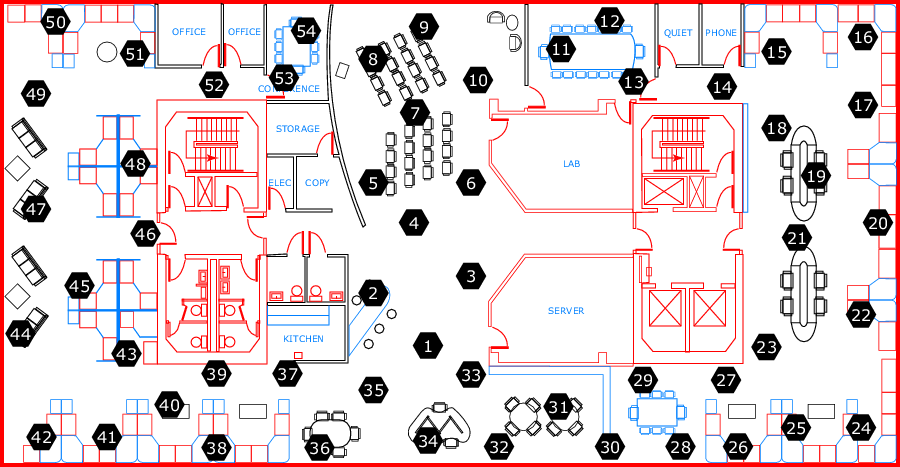
\includegraphics[scale=.25]{Figs/ibrl_wsn.png}
\caption{A map of sensors' location. (Source: \cite{Buonadonna2005})}
\label{fig:sensor_map}
\end{figure}

In this paper we consider the IBRL data set obtained from $5$ close nodes, $1, 2, 33, 35, 37$. Also, only two features, namely temperature and humidity, are taken into account. The data during the first $10$ days period on March 2004 will be used as the training set. This training set contains more than $82000$ samples and hereafter is reduced into only $55421$ samples. 

\subsection{Gaussian kernel parameter optimization}

The objective function $J(\sigma)$ according to the given training set is depicted in Fig.~\ref{fig:cost_fcn} and is evidently strongly convex.
\begin{figure}[H]
\centering
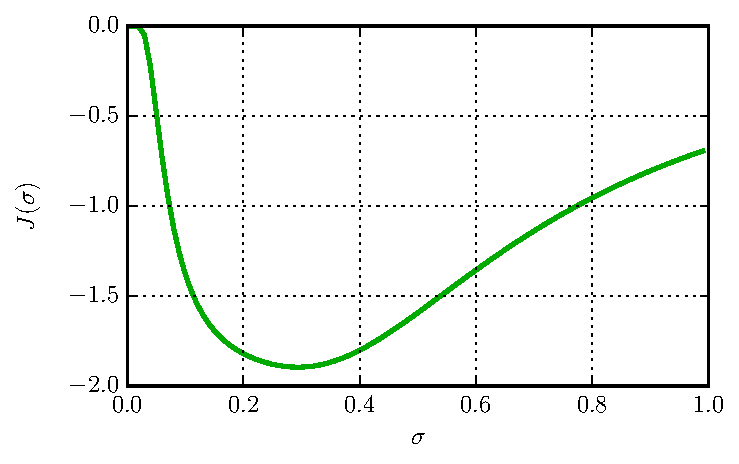
\includegraphics[scale=.6]{Python/cost_fcn.pdf}
\caption{Objective function $J(\sigma)$. }
\label{fig:cost_fcn}
\end{figure}

The Matlab's routine \emph{fminunc($\cdot$)} is used for parameter optimization, thus providing the kernel parameter $\sigma^\star=0.2938$ after few iterations.

\subsection{Training OCSVM and some results}

Using the LIBSVM library \cite{chang2011}, the OCSVM is computed with $\nu=0.0001$ and $\sigma=0.2938$, consisting only $9$ support vectors. Fig.~\ref{fig:domain_boundary} depicts the training set (green dot), the support vectors (white dot) and decision boundaries with different discriminative threshold. 
\begin{figure}[H]
\centering
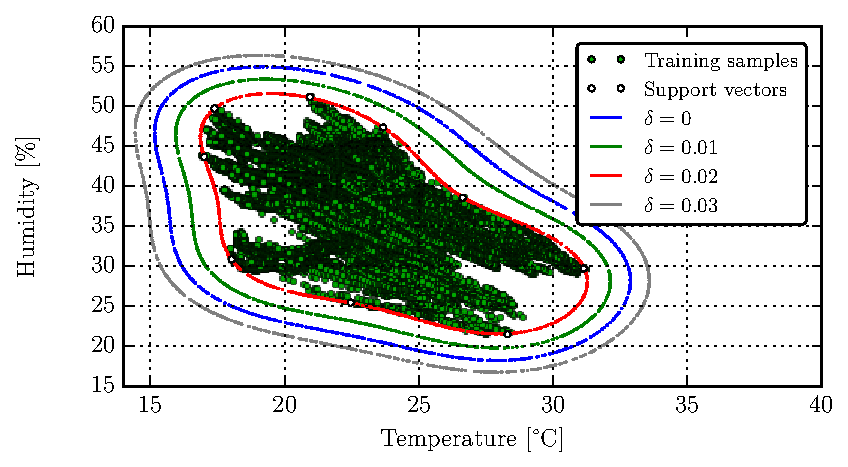
\includegraphics[scale=.6]{Python/data_description.pdf}
\caption{Discrimination boundaries with some $\delta$'s values. }
\label{fig:domain_boundary}
\end{figure}

Fig.~\ref{fig:time_valid} depicts detection result on considered nodes over time with $\delta=0.02$. Although node $37$ exhibits several false alarms, such a fault detection is unavoidable and acceptable in practice.
\begin{figure*}
\centering
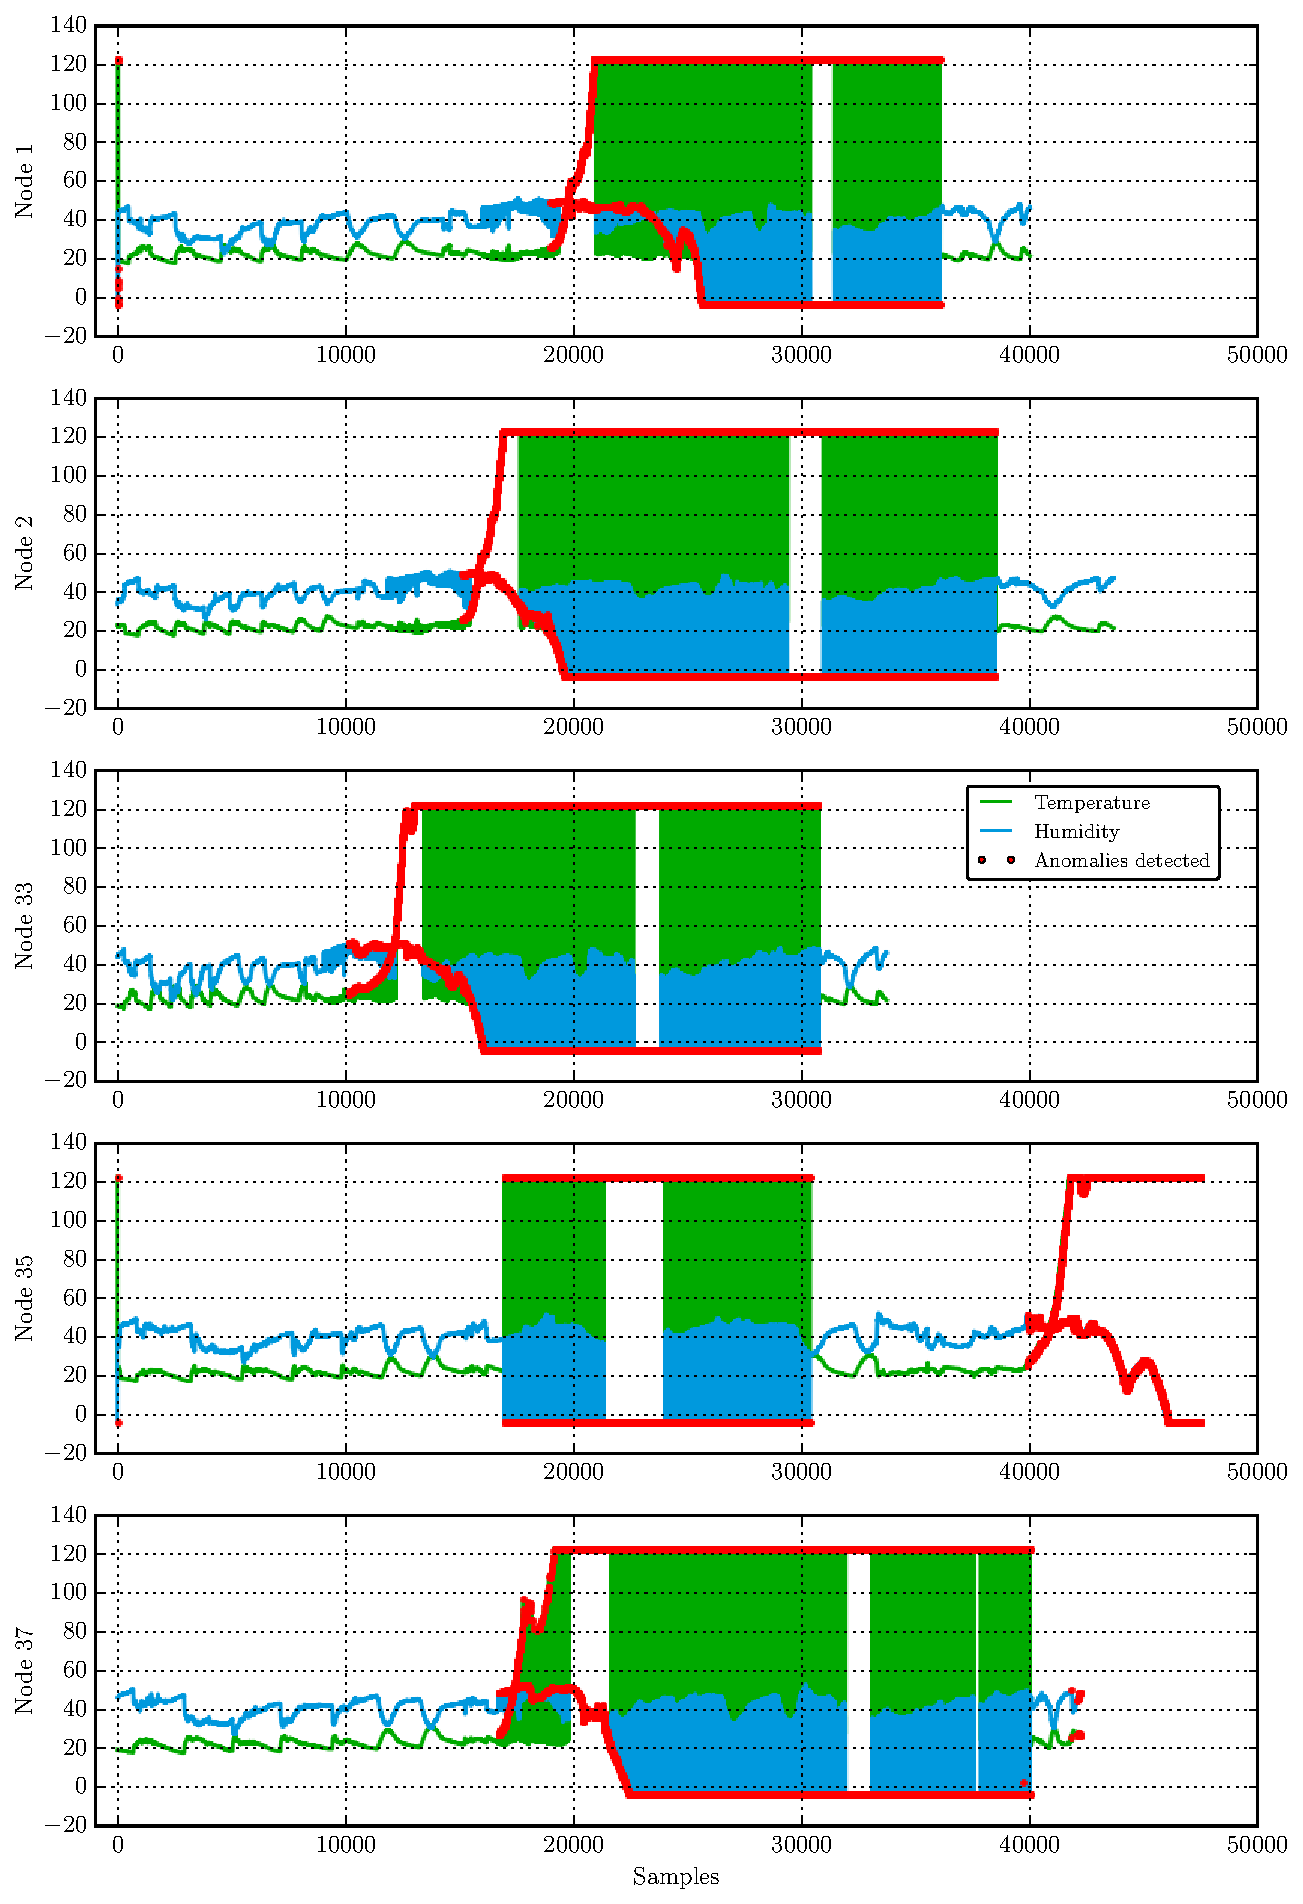
\includegraphics[scale=.7]{Python/time_validation.pdf}
\caption{Anomaly detection validation upon whole IBRL data set on $5$ nodes. Almost apparent anomalies, i.e. temperature and humidity measurements that are too high or too low, are detected. Some false alarms or non-detected anomalous measures are observed, which is acceptable in practice.}
\label{fig:time_valid}
\end{figure*}

\section{Conclusion and Future Work}\label{sec:concluding}

\bibliographystyle{plain}
\bibliography{wsnbib,svmbib,ocsvmbib,ibrlbib,miscbib}

\end{document}


